\renewcommand{\theequation}{\theenumi}
\begin{enumerate}[label=\thesection.\arabic*.,ref=\thesection.\theenumi]
\numberwithin{equation}{enumi}
\item The figure for A triangle obtained in the question looks like Fig. \ref{fig:tri_right_angle}.
with angles $\angle A,\angle C$ and $\angle B$ and sides $a, b$ and $c$.  The unique feature of this triangle is $\angle C$ which is defined to be $90\degree$.


%\renewcommand{\thefigure}{\theenumi.\arabic{figure}}
\begin{figure}[!ht]
\centering
\resizebox{\columnwidth}{!}{

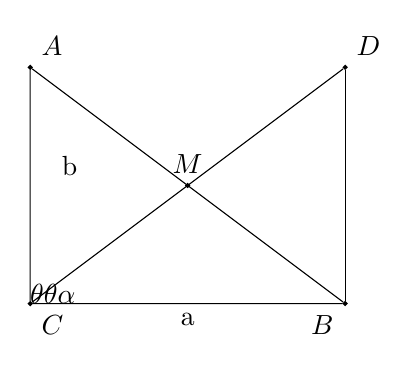
\begin{tikzpicture}
[scale=1,>=stealth,point/.style={draw,circle,fill = black,inner sep=0.5pt},]

%Triangle sides
\def\a{4}
\def\b{3}
\def\c{sqrt(\a^2+\c^2)}



%Labeling points
\node (A) at (0,\b)[point,label=above right:$A$] {};
\node (B) at (\a, 0)[point,label=below left:$B$] {};
\node (C) at (0, 0)[point,label=below right:$C$] {};
\node (M) at (\a*0.5,\b*0.5)[point,label=above:$M$] {};
\node (D) at (\a,\b)[point,label=above right:$D$] {};


%Drawing triangle ABC
\draw (A) -- node[left] {$\textrm{}$} (B) -- node[below] {$\textrm{a}$} (C) -- node[above,xshift=5mm] {$\textrm{b}$} (A);

%Joining CD
\draw (C)--(D);
%Joining BD
\draw (B)--(D);

%Drawing and marking angles
\tkzMarkAngle[fill=orange!40,size=0.5cm,mark=](A,M,C)
\tkzMarkAngle[fill=orange!40,size=0.5cm,mark=](B,M,D)
\tkzMarkAngle[fill=green!40,size=0.5cm,mark=](A,B,C)
\tkzMarkRightAngle[fill=blue!20,size=.2](A,C,B)
\tkzMarkRightAngle[fill=blue!20,size=.2](D,B,C)
\tkzLabelAngle[pos=0.65](A,M,C){$\theta$}
\tkzLabelAngle[pos=0.65](B,M,D){$\theta$}
\tkzLabelAngle[pos=0.65](A,B,C){$\alpha$}


\end{tikzpicture}
}
\caption{Right Angled Triangle by Latex-Tikz}
\label{fig:tri_right_angle}	
\end{figure}
%
%
%\renewcommand{\thefigure}{\theenumi}
%
\item List the design parameters for construction
\label{const:table1}
\\
\solution See Table. \ref{table:table1}. 
%
\begin{table}[ht!]
\centering
\begin{tabular}{ |p{3cm}|p{3cm}|  }
\hline
 \multicolumn{2}{|c|}{Initial Input Values.} \\
\hline
a & 4\\
\hline
b & 3\\
\hline
$\angle(ACB)$ & $90^{\circ}$ \\
\hline
\end{tabular}
\caption{To construct $\triangle ACB$}
\label{table:table1}	
\end{table}

%\item
%	For simplicity, let the greek letter $\alpha = \angle B$.  We have the following definitions.
%\begin{equation}
%\label{eq:tri_trig_defs}
%\begin{matrix}
	%\sin \theta = \frac{b}{c} & 	\cos \theta = \frac{a}{c} \\
	%\tan \theta = \frac{c}{a} & \cot \theta = \frac{1}{\tan \theta} \\
	%\csc \theta = \frac{1}{\sin \theta} & \sec \theta = \frac{1}{\cos \theta}
	%\end{equation}
%
\item Find the coordinates of the various points in Fig. \ref{fig:tri_right_angle}
\label{const:tri_right_angle}
\\
%
\solution From the given information, 
%$\triangle ABC$ are 
\begin{align}
\label{eq:constr_a}
\vec{A} &= \myvec{0\\b} 
\\
 \vec{C} &= \myvec{0\\0}, 
\label{eq:constr_c}
\\
\vec{B} &= \myvec{a\\0}
\label{eq:constr_b}
\end{align}
$\because \vec{M}$ is the midpoint of $AB$,
\begin{align}
\vec{M}= \frac{\vec{A}+\vec{B}}{2} = \frac{1}{2}\myvec{a\\b}
\label{eq:constr_m}
\end{align}
%
Also, $\vec{M}$ is given to be the midpoint of $C$.  Hence, 
\begin{align}
\vec{M}&= \frac{\vec{C}+\vec{D}}{2}
\\
\implies \vec{D} &= 2 \vec{M} - \vec{C} = \myvec{a\\b}
\label{eq:constr_d}
\end{align}
%
The values are listed in 
%\item List the  derived values.
%\label{const:table2}
%\\
%\solution See  
Table. \ref{table:table2} 
\begin{table}[ht!]
\centering
\begin{tabular}{ |p{3cm}|p{3cm}|  }
\hline
 \multicolumn{2}{|c|}{Derived Values.} \\
\hline
$\vec{M}$ & $$\begin{pmatrix}2\\1.5\end{pmatrix}$$\\						
\hline
$\vec{D}$ & $$\begin{pmatrix}4\\3\end{pmatrix} $$\\
\hline
\end{tabular}
\caption{To construct $\triangle DCB$}
\label{table:table2}
\end{table}
%
\item Draw Fig. \ref{fig:tri_right_angle}.	
\\
\solution The  following Python code generates Fig. \ref{fig:tri_sss_py}
%
\begin{lstlisting}
codes/triangle.py
\end{lstlisting}
\begin{figure}[!ht]
\centering
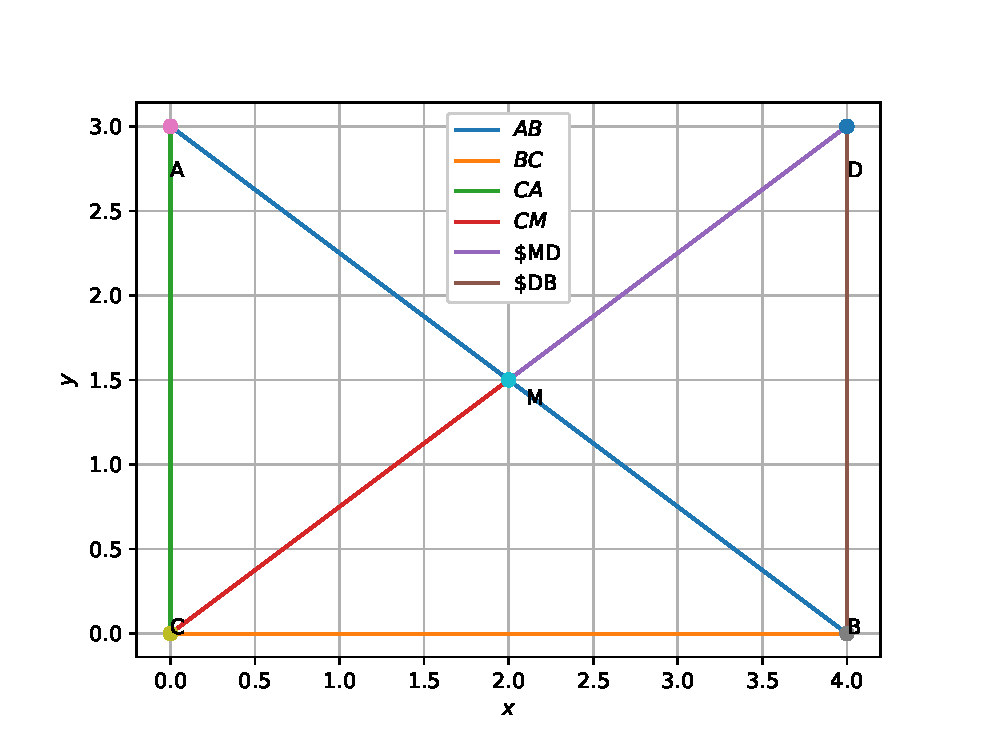
\includegraphics[width=\columnwidth]{./figs/triangle.eps}
\caption{Triangle generated using python}
\label{fig:tri_sss_py}
\end{figure}

%
and the equivalent latex-tikz code generating Fig. \ref{fig:tri_right_angle} is 
\begin{lstlisting}
figs/triangle.tex
\end{lstlisting}
%
The above latex code can be compiled as a standalone document as
\begin{lstlisting}
figs/triangle_fig.tex
\end{lstlisting}

%

%

%
%

\end{enumerate}

